
\section{Case study}
In this section, we will introduce an airplane engine control software case study. Due to its huge scale, we choose one of its subsystem, the PLA signal processing system, as representative. We will give an informal description of it, focusing on its functional structure, properties and conditional constraints. To perform deadlock freedom analysis, we generate a formal system model in BIP. Finally, we provide model verfication and validation for the system above.

\subsection{Informal description}
The Power Level Angle(PLA) signal processing system is part of the Full Authority Digital Engine Control System(FADEC), which provides engine control during flight to achieve stable and transient engine characteristics. The purpose of PLA signal processing system is to convert the obtained throttle stick signal value into the original throttle stick angle value and judge it. If it is judged that there is no fault, then it will return the corresponding value of the PLA signal after processing and set a fault signal to invalid, representing that the system has no PLA signal fault in current period. Otherwise it will return the fault information and set the fault signal to valid. The flow chart of PLA signal processing is roughly as follows:
%Picture TBD

As shown in figure ?, there are three modules in the system. PLA signals will first undergo a BIT Diagnosis module, then be calibrated and converted into physical quantities. After the Extremum and Slope Diagnosis module, it will finally generate the PLA fault signal for output.

The Built-int Test(BIT) refers to the detection and monitoring of the system and its own equipment. In the PLA signal processing system model, the BIT Diagnosis realizes the analog quantity, or periodic fault detection of circuits such as fault location and processing based on the diagnosis results.

The calibration conversion module's function is to collect the signal from signal collector. The arriving signal will be converted to the corresponding engineering value by means of a calibration curve or an index table.

An Extremum/Slope Diagnosis module contains extremum diagnosis and slope diagnosis.The function of extremum diagnosis is to judge whether the current signal is in valid range since the PLA signal processing system cannot handle illegal data. The function of slope diagnosis is to give the constraint of the magnitude of the change between the two adjacent signals.

The three modules introduced above work together for giving a credible output signal. In the next chapter, we will translate this informal model to formal BIP model for further verification and validation. 
\subsection{Formal system model in BIP}
We design our PLA Signal Processing System's BIP model through a combination between series of BIP components with BIP interactions. The block diagram for our system is shown in figure 1.

\begin{figure}[ht!]
	\centering
	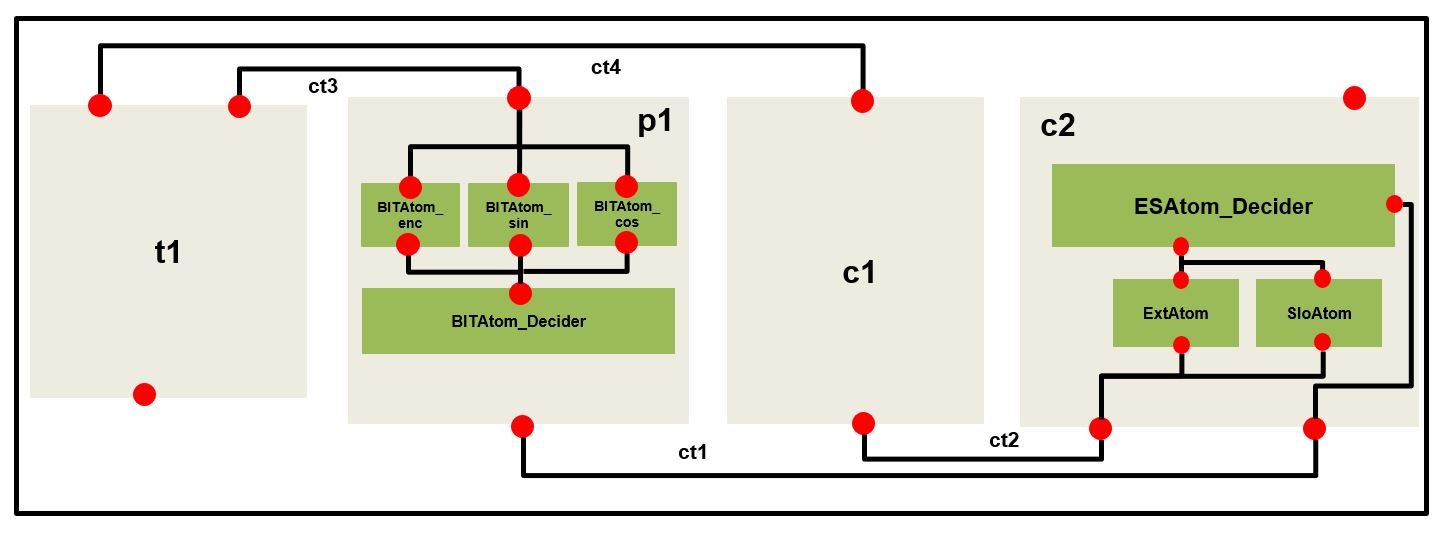
\includegraphics[width=90mm]{figure/figure2.jpg}
	\caption{Architecture of System}
	\label{Sys_Model}
\end{figure}

The atomic components of our system are \emph{TaskAtom t1}, \emph{CalibrationAtom c1} and several atomics in \emph{p1} and \emph{c2}. For each atomic component, we specify its ports, variables and behavior.

\begin{figure}[ht!]
	\centering
	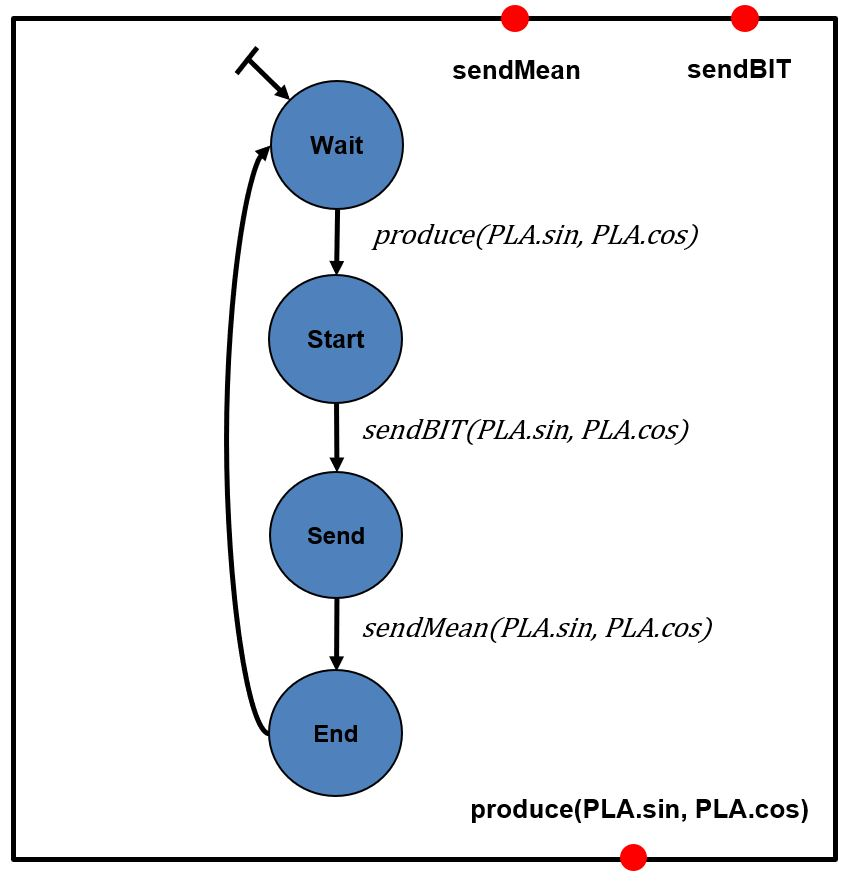
\includegraphics[width=50mm]{figure/figure3.jpg}
	\caption{The Task Component}
	\label{Task_Component}
\end{figure}

\begin{figure}[ht!]
	\centering
	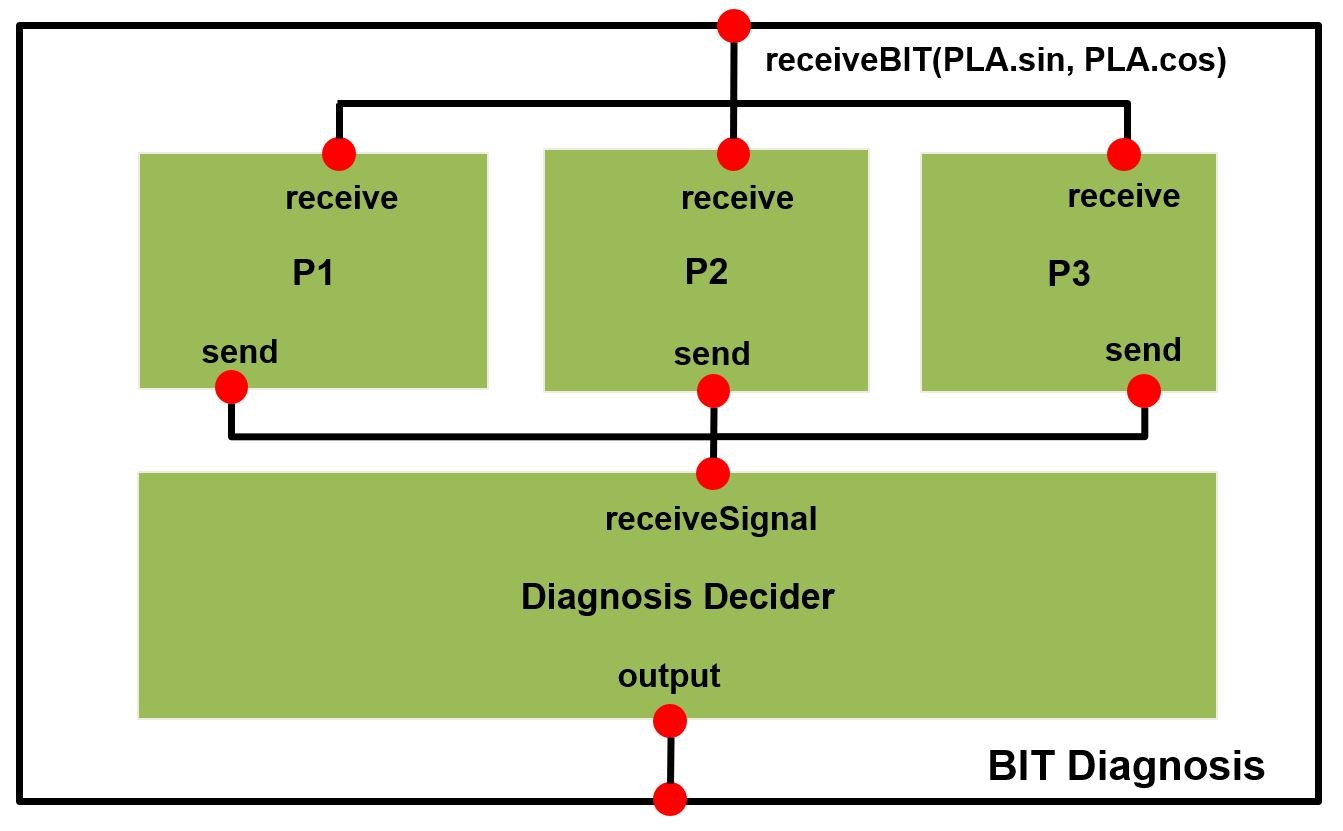
\includegraphics[width=80mm]{figure/figure4.jpg}
	\caption{Architecture of BIT Diagnosis}
	\label{BIT_Model}
\end{figure}

An atomic model of \emph{Task} is shown in figure 2, which can be used as a function of message sender in \emph{System}. In the graphical notation, the atomic is initialized to \emph{Wait}, and the following three transitions are driven by corrensponding events: \emph{produce}, \emph{sendBIT} and \emph{sendMean}, which represents three corrensponding ports in the atomic. For instance, whenever the current state is at \emph{Start}, the port \emph{sendBIT} will be activated and the transition will be executed once the event \emph{sendBIT} is done.

In our design, the BIT Diagnosis is a subsystem of PLA signal processing system. Its architecture is shown in figure 3. In the graphical notation, the three atomic component instances \emph{p1}, \emph{p2} and \emph{p3} receive BIT signal through port \emph{receiveBIT}, a connector distributes the signal to these components and another connector merges their output and sends it to the an instance of \emph{Decider} component. The BIP description of \emph{BIT Diagnosis} is shown below:

\begin{lstlisting}
`\textbf{compound} \emph{BITCompound\_P1}`
  `\textbf{component} \emph{BITAtom\_enc enc}`
  `\textbf{component} \emph{BITAtom\_sin sin}`
  `\textbf{component} \emph{BITAtom\_cos cos}`
  `\textbf{component} \emph{BITAtom\_Decider d}`
  
  `\textbf{connector} \emph{ThreeToOne o(enc.sendBIT,sin.sendBIT,cos.sendBIT,d.receiveSignal)}`
  `\textbf{connector} \emph{Merge m(enc.receiveBIT,sin.receiveBIT,cos.receiveBIT)}`
  
  `\textbf{export port} \emph{m.Merged\_Signal} \textbf{as} \emph{receiveBIT}`
  `\textbf{export port} \emph{d.output} \textbf{as} \emph{sendBIT}`
`\textbf{end}`
\end{lstlisting}

In our system, atomic component is considered as the smallest unit of the architecture, while in the combination of several components, such as our BIT Diagnosis module, we have to ensure that the output of three components can simultaneously reach the connoector, otherwise it will fall into deadlock status. To avoid this problem, the three atomic components are designed homogeneous, we take one of these three components, \emph{BITAtom\_enc p1}, as an example, its ports and behavior is shown below:

\begin{figure}[ht!]
	\centering
	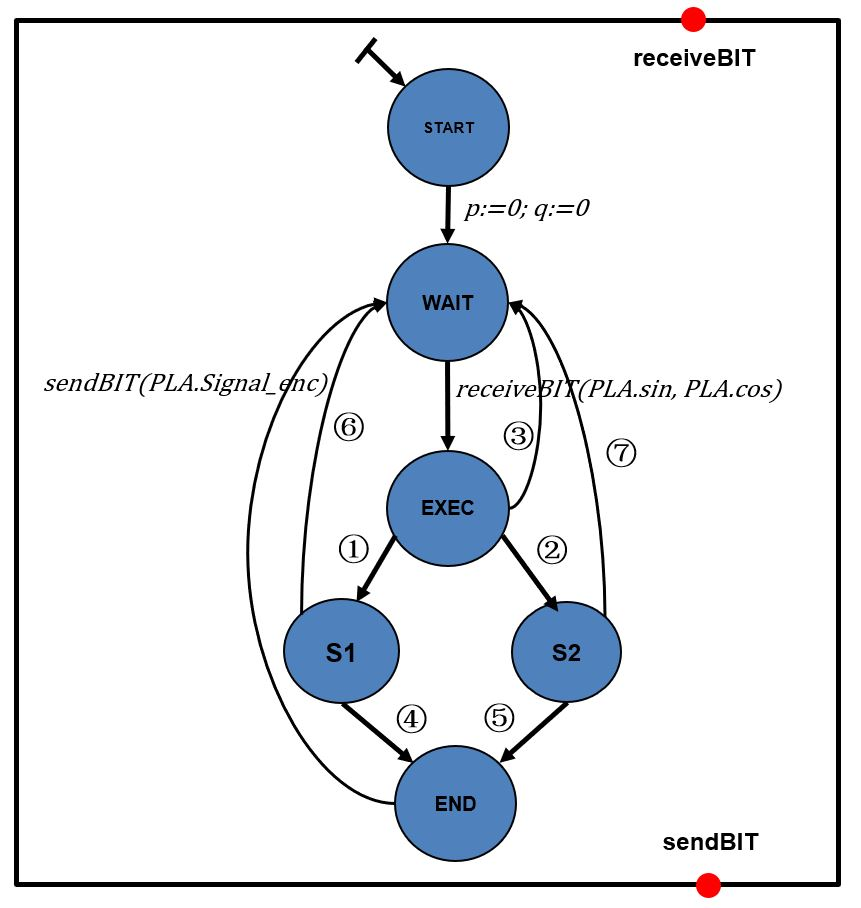
\includegraphics[width=60mm]{figure/figure5.jpg}
	\caption{Architecture of BIT Diagnosis P1}
	\label{BIT_enc_Model}
\end{figure}
\begin{table}[]
	\vspace{20pt}
	\caption{Transitions of P1}
	\centering
	\begin{tabular}{lllll}
		\hline
		\thead[l]{Transition} & \thead[l]{Guard}& \thead[l]{Action}
		\\
		\hline
		1  & PLA.sin $<500 \wedge$ PLA.cos $<500$   & $p :=p+1 ; q :=0$ \\
		2  & PLA.sin $>=500 \wedge$ PLA.cos $>=500$   & $p :=0 ; q :=q+1$ \\
		3  & PLA.sin $ >=500 \oplus$ PLA.cos $>=500$   & $p :=0 ; q :=0$ \\
		4  & $p>=5$   & PLA.Signal\_enc: $=1$ \\
		5  & $q>=5$   & PLA.Signal\_enc: $=0$ \\
		6  & $p<5$   & null \\
		7  & $q<5$   & null \\
		\hline       
	\end{tabular}
	\label{bs}
\end{table}

During execution, we consider a WAIT to WAIT transition set as a cycle. In each cycle, we ensure that an \emph{sendBIT} event will be activated to avoid the system falling into deadlock status. With the combination of connector, \emph{P1} gives a synchronous output together with other two atomic component instances. We define two variables \emph{p} and \emph{q} as counters to control the vary of signal. Their constraint indicates that for every continuous five cycles, the system does a setting and gives a corresponding output through port \emph{sendBIT}.

To give a formal proof of its safety and effectiveness. The verification and validation of the system above will produced in the next chapter.
\subsection{Model verification and validation}

